\section{MLIL Based OpenIE}

    \subsection{Major Drawback of \shortname: Speed}

        Despite achieving significant performance boost over the existing OpenIE systems, \shortname\ is not efficient for large scale use because of one major disadvantage: \emph{Speed}. Table \ref{tab:main-table} compares the different OpenIE systems on their performance as well as speed of execution. \shortname\ falls much behinds other OpenIE systems since it is able to process only 3 sentences per second.

        % TABLE: Main scores table
        \begin{table*}[h]
            
            \centering {\footnotesize
            \begin{tabular}{lccccccccccc} 
            \toprule       
            System & \multicolumn{2}{c}{CaRB} & \multicolumn{2}{c}{CaRB(1-1)} & \multicolumn{2}{c}{OIE16-C} & \multicolumn{1}{c}{Wire57-C} & \multicolumn{1}{c}{Speed}
                    \\ \cmidrule(r){2-3} \cmidrule(r){4-5} \cmidrule(r){6-7} \cmidrule(r){8-8} \cmidrule{9-9}
                   & F1 & AUC & F1 & AUC & F1 & AUC & F1 & \makecell{Sentences/sec.}     \\
                   
            \midrule                         
            MinIE           
            & 41.9 & - & 38.4 & - & 52.3 & - & 28.5 & 8.9\\
            ClausIE         
            & 45.0 & 22.0 & 40.2 & 17.7 & 61.0 & 38.0 & 33.2 & 4.0\\
            OpenIE-4            
            & 51.6 & 29.5 & 40.5 & 20.1 & 54.3 & 37.1 & 34.4 & 20.1\\
            OpenIE-5            
            & 48.0 & 25.0 & 42.7 & 20.6 & 59.9 & 39.9 & 35.4 & 3.1\\
            \midrule
            SenseOIE        
            & 28.2 & -    & 23.9 & -    & 31.1 & -    & 10.7 & - \\
            SpanOIE         
            & 48.5 & -    & 37.9 & -    & 54.0 & -    & 31.9 & 19.4\\
            RnnOIE          
            & 49.0 & 26.0 & 39.5 & 18.3 & 56.0 & 32.0 & 26.4 & \textbf{149.2}\\
            \cite{cui+18}      
            & 51.6 & 32.8 & 38.7 & 19.8 & 53.5 & 37.0 & 33.3 & 11.5\\
            IMoJIE (Agg)
            & 53.5 & 33.3 & 41.4 & 22.2 & 56.8 & 39.6 & 36.0 & 2.6\\
            IMoJIE (OIE4) 
            & 53.2 & 33.1 & 42.2 & 22.8 & 56.1 & 38.1 & 34.9 & 2.6\\
            \shortname &
            52.5 & 32.0 & 41.0 & 21.7 & 55.5 & 35.0 & 35.1 & 157.1 \\
            \shortname(CL) & 
            \textbf{54.2} & \textbf{34.2} & 43.0 & 23.3 & 59.4 & 39.1 & 37.1 & 157.1 \\
            % \shortname~(CL) + Rescore &
            % \textbf{54.2} & \textbf{34.5} & 43.1 & 23.4 & 59.5 & 42.5 & 37.1 & 100.1 \\
            % \shortname~(CL) + \shortname-CA & 
            % 51.6 & 31.0 & 45.3 & 24.7 & \textbf{65.4} & 45.1 & 39.6 & 95.0 \\
            \shortname(CL) + \shortname-CA &
            52.7 & 33.7 & \textbf{46.2} & \textbf{26.6} & \textbf{65.1} & \textbf{48.0} & \textbf{40.2} & 83.0 \\
            
            % \shortname
            % & 52.2 & 32.7 & 40.7 & 21.6 & 55.3 & 38.3 & 34.8 & 100.1\\
            % \shortname+CL
            % & \textbf{53.7} & \textbf{34.0} & 42.8 & 23.1 & 59.1 & 42.2 & 36.8 & 100.1\\
            % \shortname+CL (no re-scoring)
            % & \textbf{53.7} & \textbf{34.0} & 42.8 & 23.1 & 59.1 & 42.2 & 36.8 & 142.8\\
            % \shortname+CL+CA
            % & 52.7 & 33.7 & \textbf{46.2} & \textbf{26.6} & \textbf{65} & \textbf{47.9} & \textbf{39.8} & 71.4\\
            % \shortname+CL+CA (no re-scoring)
            % & 52.2 & 33.1 & \textbf{45.9} & \textbf{26.3} & \textbf{65} & \textbf{47.9} & \textbf{39.8} & 95.0\\
            \bottomrule
            \end{tabular}
            \caption{Evaluation of OpenIE. Using constrained learning, \shortname(CL) offers a 60x speedup and better performance scores on all metrics compared to IMoJIE. Adding a coordination analyzer, \shortname(CL) + \shortname-CA gives the best scores in 3 of the 4 metrics. MinIE, SenseOIE, SpanOIE do not output confidences. Code of SenseOIE is not available to compute speed.}
            \label{tab:main-table}
            }
        \end{table*}
        
        % reasons for slow speed
        The low speed of execution of \shortname\ is attributed to its high computational cost which comes by virtue of its iterative generation proceduce. \shortname\ is a state-of-the-art OpenIE system that re-encodes the partial set of extractions so far when generating the next extraction. This captures dependencies among extractions, reducing the overall redundancy of the output set. However, this repeated re-encoding causes a significant reduction in speed, which limits use at web scale.

        On the other hand, \emph{labeling}-based systems like RnnOIE \citep{stanovsky&al15} are much faster (150 sentences per second, compared to 3 sentences of IMoJIE) but relatively less accurate. They label each word in the sentence as either \textit{S} (Subject), \textit{R} (Relation), \textit{O} (Object) or \textit{N} (None) for each extraction. However, as the extractions are predicted independently, this does not model the inherent dependencies among the extractions.

        The challenge at hand now is to bridge this gap by a system that is both fast and accurate.

    \subsection{OpenIE as 2-D Grid Labelling}

        \begin{figure}[h]
            \centering
            % 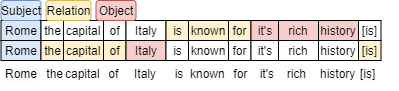
\includegraphics[width=8cm,height=1.5cm]{images/mlil/openie_example.png}
            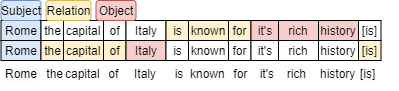
\includegraphics[width=0.8\hsize]{images/mlil/openie_example.png}
            \vspace*{-4ex}
            \caption{The extractions \textit{(Rome; [is] the capital of; Italy)} and \textit{(Rome; is known for; it's rich history)} can be seen as the output of the grid labeling. We additionally introduce a token \textit{[is]} to the input.}
            \label{fig:grid_example}
        \end{figure}

        We present a novel labelling-based architecture, \mlilboldlongname~(\mlilboldshortname), which models OpenIE as 2-D grid labeling problem of size $(M, N)$ where $M$ is a pre-defined maximum number of extractions and $N$ is the sentence length, as shown in Figure~\ref{fig:grid_example}.

        Each extraction corresponds to one row in the grid. Iterative assignment of labels in the grid helps \mlilshortname\ capture dependencies among extractions without the need for re-encoding. This makes it 25 times faster (80 sentences per second) than IMoJIE.

        While \mlilshortname\ gives high precision, we can further improve recall by incorporating (soft) global coverage constraints on this 2-D grid. We use constrained training \citep{mehta&al18} by adding a penalty term for all constraint violations. This encourages the model to satisfy these constraints during inference as well, leading to improved extraction quality, without affecting running time.


\section{Coordination Analyzer}

    Furthermore, the existing neural OpenIE models struggle in handling coordination structures, and do not split conjunctive extractions adequately. In response, we first design a new coordination analyzer \citep{ficler&goldberg16b}. It is built with the same \mlilshortname~ architecture, by interpreting each row in the 2-D grid as a coordination structure. This leads to a new state of the art on this task, with a 13 pt improvement in F1 over previous best reported result \citep{teranishi+19}, and a 2.5 pts gain in F1 over a strong BERT baseline. 

    We then combine the output of our coordination analyzer with our OpenIE system, resulting in a further increase in performance (Table~\ref{tab:redundancy-example}). We evaluate our final OpenIE system on four metrics from the literature and find that it exceeds in three of them by at least 4.2 pts in F1.
    
    We undertake manual evaluation to reaffirm the gains. Two annotators, blind to the underlying systems, independently label each extraction as correct or incorrect for a subset of 100 conjunctive sentences. Their inter-annotator agreement is 93.46\%. After resolving the extractions where they differ, we report the precision and yield in Table \ref{tab:manual_annotation}. Here, yield is the number of correct extractions generated by a system. It is a surrogate for recall, since its denominator, number of all correct extractions, is hard to annotate for OpenIE.  

    We find that \mlilshortname(CL)+CA significantly increases the yield (1.7x) compared to \mlilshortname(CL) at a marginal increase in precision. This result underscores the importance of splitting coordination structures for OpenIE. Our final OpenIE system, \mlilshortname(CL)+CA, is 25x faster than IMoJIE.

    \begin{table*}[h]
        \centering {\footnotesize
        \begin{tabular}{lccccccc}
        \toprule
        System                    
        & Precision & Yield & \makecell{Total\\Extrs}\\
        \midrule       
        \shortname(CL)
        & 77.9 & 131 & 174 \\
        \shortname(CL) + MLIL-CA
        & \textbf{78.8} & \textbf{222} & \textbf{291} \\
        \bottomrule
        \end{tabular}}
        \caption{Manual comparison of Precision and Yield on 100 random conjunctive sentences from CaRB Gold.}
        \label{tab:manual_annotation}
    \end{table*}

%%%%%%%%%%%%%%%%%%%%%%%%%%%%%%%%%%%%%%%%%%%%%%%%%%%%%%%%%%%%%%%%%%%%%%%%%%%%%%%%%%%%%%%%%%%%%%%%
% Uncategorised
%%%%%%%%%%%%%%%%%%%%%%%%%%%%%%%%%%%%%%%%%%%%%%%%%%%%%%%%%%%%%%%%%%%%%%%%%%%%%%%%%%%%%%%%%%%%%%%%



%%%%%%%%%%%%%%%%%%%%%%%%%%%%%%%%%%%%%%%%%%%%%%%%%%%%%%%%%%%%%%%%%%%%%%%%%%%%%%%%%%%%%%%%%%%%%%%%
% TABLES
%%%%%%%%%%%%%%%%%%%%%%%%%%%%%%%%%%%%%%%%%%%%%%%%%%%%%%%%%%%%%%%%%%%%%%%%%%%%%%%%%%%%%%%%%%%%%%%%